\chapter[Big Data Analytics Platform]{Concept and Implementation of Big Data Analytics Platform}
\label{chapter:platform}
We have referred to big data platform concept and implementation on many occasions in previous chapters. In chapter \ref{chapter:background} we have discussed the basic concepts of big data with various technological advancements and solutions available for handling big data. In chapter \ref{chapter:method} we mentioned the functional components and their implementation during different stages, cycles and iterations. In this chapter we shall first explain the concept and a sample application framework for a big data platform based on available open source components. Then we shall present the part of this concept that we have implemented for handling the energy and social media data for our energy efficiency use cases listed in section \ref{use_cases} of previous chapter. 

Before we move to our conceptual model of the big data platform it is important that we mention basic challenges that drive the design of a big data solution and briefly explain a typical big data analytics process.

\section{Big data challenges}
As discussed in section \ref{bigdata_intro} of chapter \ref{chapter:background} there are five main challenges that influence the solution design criteria for big data analytic systems. These challenges are generally termed as 5V s of big data.
\begin{enumerate}
\item \textbf{Volume} refers to the size of the data. Volume is the most commonly associated feature with the big data. The big data analytics platform in our scope of work is based on Hadoop File Systsem (HDFS) which is a highly scalable system. It has been tested with upto 4000 scaled out serving nodes capable of handling upto 10 Petabytes (PB) of data.
\item \textbf{Velocity} refers to the data procesing speed.Velocity is crucial for the business use cases that need to process huge volumes of data in real time to produce insights for decision making. Our model is designed for batch processing, however we have integrated additional components that can process the data with near to real time capability.
\item \textbf{Variety} refers to structure of the data. Traditionally the relational data base system can store data with fixed schema. The fixed schemas mean that the stored data must have a definitive structure. Such databases are designed on basis of these data structures. In context to big data sometimes it is hard to perceive the structure of data so the storage systems needs to be designed for data in any structural format i.e. structured, unstructured or semi-structured formats. In our conceptual model we have added various components that can handle all formats of the data. However, In our implementation we shall be processing the data that had known fixed schema. 
\item \textbf{Veracity} refers to the complexity due to noises and inconsistencies of the data. In real life scenarios for big data it is very rare to find data in absolute consistent. Most of the time some values will be missing or the data will be in wrong format or there will pollutions in data. For good analysis we need to take care of such inconsistency and errors in data. Our conceptual model is capable of handling inconsistencies and in our implementation we had catered for some inconsistencies that we shall discuss in next chapter \ref{chapter:Analysis}. 
\item \textbf{Valuation} refers to the benefits of processing big data against the efforts required. It is an emerging feature for big data analysis design. Just like the other IT systems, organizations tends to decide about big data investments by looking at the business cases. In our concept we shall be discussing a model based on open source components. So there should be no cost of acquiring software. There is no specialized hardware requirements for implementing our model and any commercially available hardware with moderate specifications can be used to deploy this software. Hardware maintenance is required for running the service based on our model. However their are cloud alternatives that can be use within our model with some costs. However we shall not be discussing such alternatives in scope of this document or our research.    
\end{enumerate} 
\section{Data Analysis work-flow}
 The data analysis process involves collection of data from multiple heterogeneous sources including both social media data, consumer data, sensors data, and already data from data servers or databases etc. The collected data in its original form can be ingested directly into Hadoop file system (HDFS). If required some filters can also be applied while collecting the data for efficient use of storage space. Collected data can be structured, semi structured or unstructured and some pre processing can be done to format it i.e. form a schema or structure that can be stored and accessed for data mining in database(s). A data mining engine with flexibility to plug and use various quantitative and qualitative research tools can then be used to analyse the data as per use case requirements. Data mining engine requires a feedback loop to pre-processing unit to adapt to the requirements of the use cases. Another feedback channel for processed data storage can be provided for direct data manipulations. Results of the data mining can be stored in the database. A RESTful API or data driver can be used to extract data from database for visualization frontends. Figure~\ref{fig:process} shows the high level process flow.
 \begin{figure}[!h]
   \begin{center}
     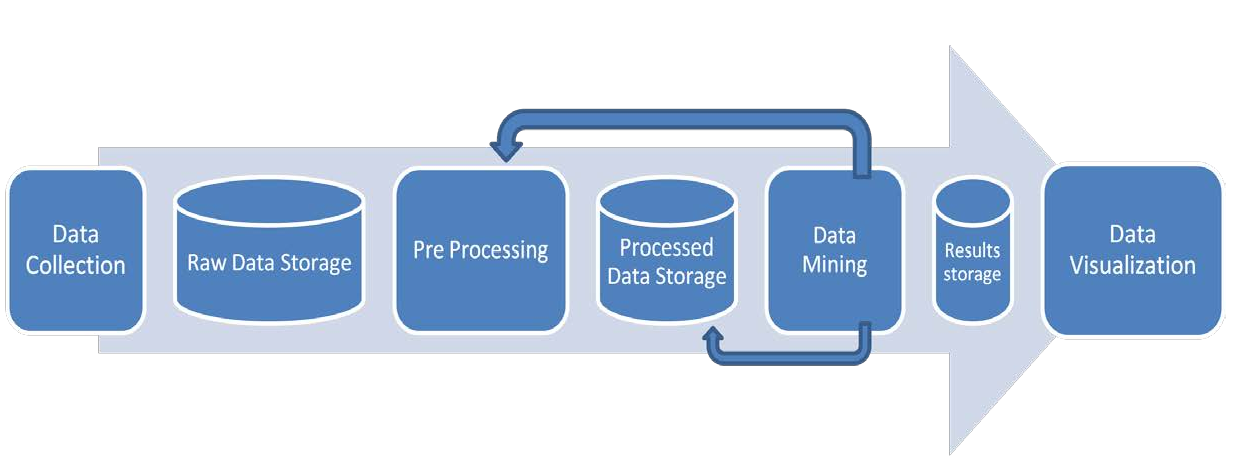
\includegraphics[width=\textwidth]{images/process.pdf}
     \caption{High level data processing flow.}
     \label{fig:process}
   \end{center}
 \end{figure} 
 \section{Platform concept}
 This section presents an end to end big data analytics platform aligned with the data processing flow described in previous section. The proposed platform is based on software components that are available open source free of cost. However use of each software components is subjected to its respective license under a specific open source licensing scheme. There are closed source and paid cloud services components available that can be used as efficient alternatives for parts of this model. However this paper does not contain information about these alternatives. Figure ~\ref{fig:cplatform} illustrate the proposed concept
 \begin{figure}[!h]
    \begin{center}
      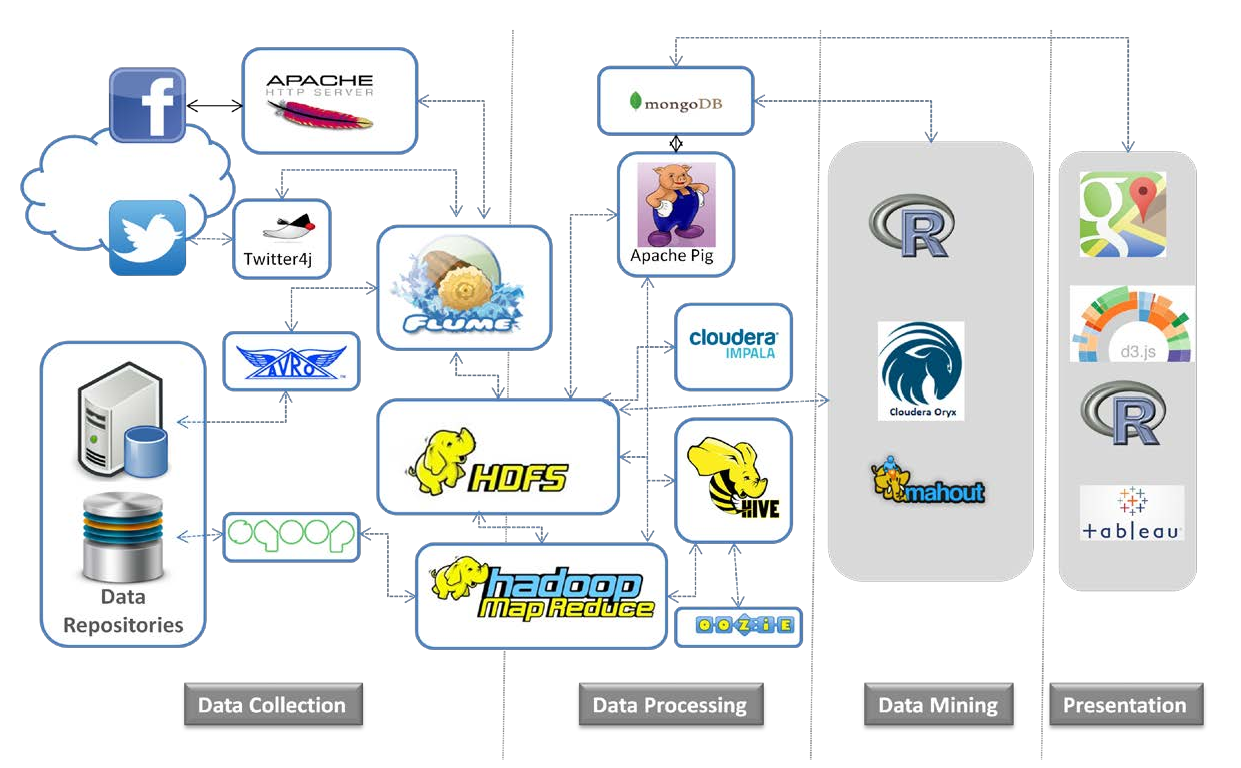
\includegraphics[width=\textwidth]{images/cplatform.pdf}
      \caption{Conceptual model of big data analytics .}
      \label{fig:cplatform}
    \end{center}
  \end{figure} 
\section{Data Core}
Before we go into details of each and every process step and respective components, it is beneficial to discuss the data core of the platform that is based on Apache Hadoop MapReduce and the Hadoop file system (HDFS).These two components are also shared between data collection and data processing steps.  Apache Hadoop is a framework that allows the distributed processing of large data sets across clusters of computers and HDFS is a distributed file system that provides high throughput access to application data\cite{apachehadoop} thus providing a highly efficient and scalable solution for handling big data. We have described Hadoop and MapReduce in section \ref{mapr}.
\section{Data Collection}
The proposed platform is capable of collecting and aggregating data from multiple data streams i.e social media data, consumer data, or server log files etc. The data can be live streaming data or data residing in server file systems or databases. Data can be collected as it is so there are no dependencies on format or structure of the data. Some filtering can also be applied while collecting data e.g. collecting only the geo tagged tweets or collecting logs with error notifications only. Following two components are recommended for data collection
\subsection{Apache Flume}
Apache Flume is a distributed service for efficiently collecting, aggregating and moving large amount of data \cite{flume}. Multiple flume agents can be configured to collect data from heterogeneous sources, channel the data to configurable destinations and store on desired locations. In the proposed model Apache flume is using Twitter4j library to stream data from Twitter, Apache HTTP REST API for collecting Facebook data and Apache Avro\cite{avro} data serialization system to collect log data from file systems of remote servers. Flume is then ingesting data directly into hadoop file system (HDFS). Flume can also read from databases and it is particularly useful while reading from document stores (NoSQL databases). However for reading from relational databases Apache foundation has another useful tool called Sqoop.
\subsection{Apache Sqoop}
Apache Sqoop \cite{sqoop} is designed for efficiently transferring bulk data between relational databases and Hadoop. So in most of the consumer data cases Sqoop can be used to collect data and feed it into HDFS through running multiple parallel Hadoop MapReduce jobs.
\section{Data Pre-processing}
Once the data is available in HDFS then it can be normalized to definitive structured forms e.g. schema. Furthermore, certain filtering can be applied for example in case of tweets, tweet text can be separated from other information for qualitative analysis and then natural language processing techniques can be applied to get it ready for further text mining. Usually pre-processing also helps in filtering out the unwanted information and make data lighter for mining process. In the proposed model Apache Pig and Hive are used to pre-process the data. Apache pig and hive both use Hadoop Mapreduce as parallel batch processing. For sake of fast pre-processing Cloudera Impala is also also added to the model.
\subsection{Apache Hive}
Apache Hive \cite{hive} is data ware house software that provides a way of providing schema to the stored data with SQL based query language to extract, transform and load data (ETL). Apache hive is further supported by another Apache Hadoop ecosystem tool called Oozie. Ooozie is acting as a workflow scheduler for Hadoop i.e. while loading the data into Hive it can create partition for tables arrange the data for optimized querying.
\subsection{Apache Pig}
Apache Pig \cite{pig}  provides a high level scripting language to analyze the data stored in HDFS using MapReduce. 
\subsection{Cloudera Impala}
